\documentclass[a4paper,english]{article}
\usepackage{graphicx}
\usepackage[T1]{fontenc}
\usepackage[utf8]{inputenc}
\usepackage{babel}
\usepackage[colorlinks=true]{hyperref}
\usepackage{upgreek} %proper greek letters
\usepackage{fullpage}
\usepackage{lineno}
\usepackage{amsmath} % typesetting math
\usepackage{amssymb}
\usepackage{booktabs} % nice tables
\usepackage[round,sort&compress]{natbib}
\usepackage{pdfpages} %include external pdfs
\usepackage{enumitem} %for noitemsep in lists
\usepackage{csquotes} %for noitemsep in lists
\usepackage{subfig}
\renewcommand{\arraystretch}{1.2} % space in tables
\usepackage{authblk}
\usepackage{multirow}

% \usepackage[toc,page]{appendix} %for appendix titles
% \usepackage[titletoc,title]{appendix} %for appendix titles
\usepackage[colorinlistoftodos,prependcaption,textsize=tiny]{todonotes} %todo note in margin

\begin{document}

\title{Comparison of Multi-Parallel Slit and Knife-Edge Slit Prompt Gamma Cameras in the context of hadrontherapy verification}

\author[1,2]{Brent F. B. Huisman}
\author[2]{\'E. Testa}
\author[1]{D. Sarrut}
\affil[1]{~CREATIS, Universit\'e de Lyon; CNRS UMR5220; INSERM U1206; INSA-Lyon; Universit\'e Lyon 1; Centre L\'eon B\'erard, Lyon, France}
\affil[2]{~IPNL, Universit\'e de Lyon; CNRS/IN2P3 UMR5822; Universit\'e Lyon 1 Lyon, France}
\affil[ ]{~E-mail: brent.huisman@cern.ch}

\maketitle

\begin{abstract}

\emph{Purpose:} 

\emph{Materials and Methods:} 

\emph{Results:} 

\emph{Conclusion:} 

\end{abstract}

\tableofcontents

\newpage

%%%%%%%%%%%%%%%%%%%%%%%%%%%%%%%%%%%%%%%%%%%%%%%%%%%%%%%%%%%%%%%%%%%%%%%%%%%%%%%%
\section{Introduction}

The well-defined range of particles in matter is the main reason they are used in cancer treatment today. Unfortunately we are not able to take full advantage of this property, because of uncertainties in patient positioning, the proton range, patient anatomy, and the Hounsfield unit to particle stopping power conversion \citep{Paganetti2012}. Often, medical practice is to plan conservatively, namely adding margins around the tumor, greatly reducing the potential benefits of particle treatment \citep{Knopf2013}. Online monitoring would make measurements of uncertainties such as mentioned above possible, and thereby permit more precise planning which could take maximum advantage of the steep BP fall-off and reduce damage to tissues surrounding the tumor. A new way to perform monitoring is to use prompt gammas (PGs), a natural byproduct in particle treatments and are of prime interest \citep{Moteabbed2011,Gueth2013,Golnik2014a,Janssen2014}. A knife-edge PG camera \citep{Perali2014,Richter2016} was put into clinical operation in fall 2015, at OncoRay in Dresden, Germany. The aim of such collimated cameras is to obtain a 1D profile of the PG production along the beam direction and obtain the position of the fall-off of the signal, which is strongly correlated to the BP position. Other approaches include detection of the target materials using a spectral PG camera \citep{Verburg2014}, using the primary particle's time of flight (ToF) in a timed PG measurement \citep{Golnik2014a} and Compton camera designs \citep{Roellinghoff2011,Kurosawa2012,Solevi2016,Thirolf2016,Polf2015,Llosa2016}.

To date two publications have attempted to perform an in-depth comparison between two collimated PG camera designs. \cite{Smeets2016} showed an experimental comparison of the knife-edge camera with a non-optimized CLaRyS MPS camera (some technical constraints prevented the authors to use the \enquote{optimal CLaRyS design}. In \cite{Lin2017} a MC comparison is executed on their own two collimator designs. Although the aforementioned studies may give the impression to provide a fair comparison (use of the same absorbers, same beam-collimator and collimator-absorber distance in the case of \cite{Lin2017}), they do not provide a thorough justification of their sets of parameters. Surprisingly, some parameters are even not the same between the two camera types. While it can be understood in \cite{Smeets2016} due to experimental constraints, it is more questionable in \cite{Lin2017} (different energy deposition selection).

While very interesting, such comparisons could be supported by more theoretical considerations on the expected output and camera parameters. Taking a step back, the 1D PG signal can be paramatrized, as well as the relevant dimensions of the PG collimator, the event selection criteria. A simple model could be built relating these factors which in turn can be tested in a study.

This publication will demonstrate and validate a model for a knife-edge slit (KES) and multiparallel slit (MPS) collimator designs, both analytically and by using Monte Carlo (MC) studies. The objectives of the present paper are the following:

\begin{itemize}
  \item Develop an analytical model based on geometric considerations
  \begin{itemize}
  	\item The model should allow for a theoretical estimation of the detection efficiency and spatial resolution, for both MPS and KES and so allow for conclusions to be drawn about the intrinsic features of MPS and KES collimators.
    \item Validate the analytical model using MC studies.
    \item Address deficiencies in previous studies. In \cite{Smeets2016} and \cite{Lin2017}: the KES/MPS detection efficiency ratio is 1.6 for Smeets 2016 and 5.3 for Lin 2017, assuming the use of the same energy window\todo{was it the same energy window?}. These comparision were not performed under identical conditions, nor were differences accounted for in another way.
  \end{itemize}
  \item Prototype comparison
    \begin{itemize}
    	\item The clinically relevant parameter is, currently, the fall-off position (FOP), allowing for a BP verification. The prototypes will thus be compared on that merit.
    \end{itemize} 
  
\end{itemize}  

%%%%%%%%%%%%%%%%%%%%%%%%%%%%%%%%%%%%%%%%%%%%%%%%%%%%%%%%%%%%%%%%%%%%%%%%%%%%%%%%
%%%%%%%%%%%%%%%%%%%%%%%%%%%%%%%%%%%%%%%%%%%%%%%%%%%%%%%%%%%%%%%%%%%%%%%%%%%%%%%%
%%%%%%%%%%%%%%%%%%%%%%%%%%%%%%%%%%%%%%%%%%%%%%%%%%%%%%%%%%%%%%%%%%%%%%%%%%%%%%%%

\section{Materials and Methods}

\subsection{Analytical model for spatial resolution and detection efficiency}

Camera performance is mainly characterized by a compromise between spatial
resolution and detector efficiency. During camera design, modifications of some
geometrical parameters, such as collimator-crystal distance, collimator pitch or
depth ..., often lead to improvement of one of this criteria and deterioration
of the other. Indeed, in order to compare performance of different camera types
and configurations, we derive an analytical model that roughly predict camera
performance. Two models are derived, one for Multi Parallel Slit (MPS) and one
for Knife Edge Slit (KES) collimators. Such models allow to estimate variation
in performance according to variation in geometrical parameters. The models will
be evaluated against Monte-Carlo simulations in next sections. 

The figure~\ref{fig:GeomSchemes} first defines several generic geometrical
parameters, namely: $d_1$ the source to MPS-collimator distance, $d_2$ the
MPS-collimator to crystal distance, $D$ the MPS-collimator depth, $d_3$ the
source to KES-collimator center distance, $d_4$ the KES-collimator center to
crystal distance, $L_{MPS}=d_1+D+d_2$ or $L_{KES}=d_3+d_4$ the total
source-crystal distance, $H$ the camera height, $p$ the collimator pitch, $f$
the fill factor (ratio between septa width and the pitch), $s$ the slit width
and $\alpha$ the KES-collimator angle. \todo{update the fig with p, H etc} All
distance values are in millimeters.

\begin{figure}[htbp]
    \centering
    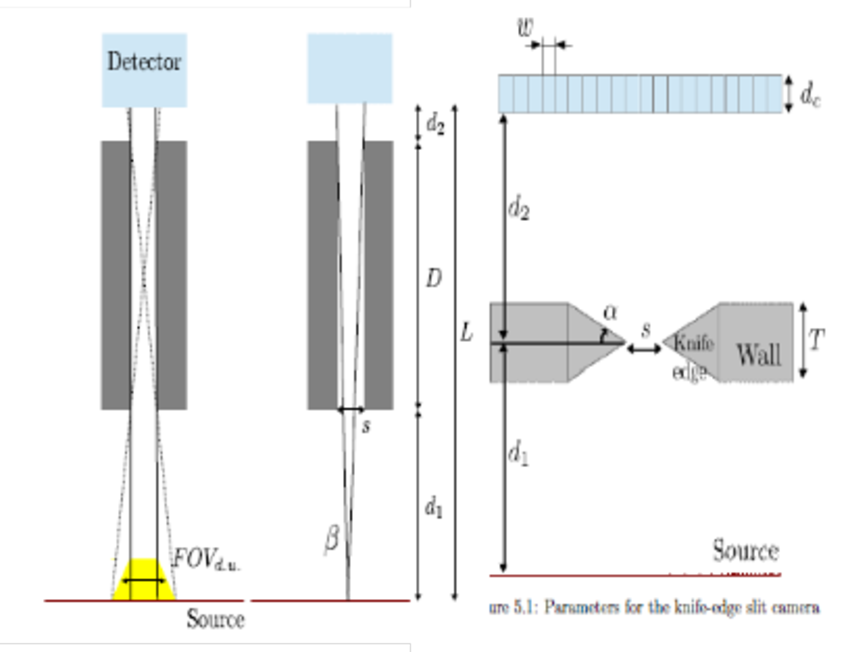
\includegraphics[width=.45\textwidth]{SchemeMPS-KES}
    \caption{Schemes of MPS and KES cameras. }
    \label{fig:GeomSchemes}
\end{figure}    
\todo{Etienne: todo => make an original figure,Change notation d1 MPS is not d1 KES. Use d1, d2, D MPS and d3 d4 for KES}      

\subsubsection{Spatial resolution}

\newcommand\FOV{\textrm{Res}\,}
\newcommand\MPS{\textrm{MPS}}
\newcommand\KES{\textrm{KES}}
%\newcommand\du{\textrm{du}}
\newcommand\du{}
\newcommand\DE{\textrm{Eff}\,}

From a geometrical point of view, the spatial resolution is characterized by the
\textit{detector unit field of view}, denoted $\FOV_{\du}$. This is the portion of
the source that can be seen through a single camera unit: a single slit for the
MPS and a single detector unit for KES. The probability of a photon emitted at a
given point along a linear source perpendicular to the slit plane to reach
this detector unit can be described as a trapezoid: the part that can be seen
from every points on the detector unit and the penumbra. We defined $\FOV_{\du}$
as the FWHM of this trapezoid, see eq~\ref{eq:fov_mps} and \ref{eq:fov_kes}.

\begin{eqnarray}
  \label{eq:fov_mps}
  \FOV_{\du}^{\MPS} & = & s\left(1+ \frac{d_1}{d_2}\right) = p(1-f) \frac{D+d_1}{D} \\
  \label{eq:fov_kes}
   \FOV_{\du}^{\KES} & = & s\left(1+ \frac{d_3}{d_4}\right) = \frac{sL}{d_4}
\end{eqnarray}

If collimator transparency is neglected, $\FOV_{\du}$ is fully defined by
geometrical parameters, in particular the slit width $s$. However, prompt gamma
have high penetration capability that can not be neglected especially in the
case of KES where the collimator depth is very small in the region of the knife
edge around the slit. Indeed, we define the \textit{Effective Slit Opening}
$s_e$ that can be used in the evaluation of the field of view and the efficiency
in place of the geometrical slit width. Metzler et al.~\cite{Metzler2005}
proposed a method to estimate the effective slit width, specifically to calculate
the spatial resolution accurately. The proposed expressions were based on
one-dimensional cuts through the pinhole geometry and can be applied directly to
a knife-edge geometry without modification. Their approach is for a point source
and dependent on the location of the source within the \FOV. For a source in the
center, it simplifies to eq.~\ref{eq:se} with $\mu$ the linear attenuation
length of the radiation in the collimator material. \todo{Why not se for MPS ?}
\todo{Add alpha and mu in the figure}.

\begin{eqnarray}
  s_e & = & s + \frac{\ln2}{\mu\tan\alpha}   \label{eq:se} \\
   \FOV_{\du}^{\KES} & = & s_e\left(1+ \frac{d_3}{d_4}\right) = \frac{s_eL}{d_4}          
  \label{eq:fov_kes_se}
\end{eqnarray}

Hence, eq.~\ref{eq:fov_mps} and eq.~\ref{eq:fov_kes_se} represent the spatial
resolution of the two KES and MPS camera systems according to simple geometrical
parameters (collimator distances, angle and collimator linear attenuation
length). The spatial resolution is expressed in millimeters. 

\subsubsection{Detection efficiency}

The probability that a photon emitted from a point facing a slit to reach the
detector is described by the solid angle $\Omega\,_D$ from that point to the
detector. For MPS, the solid angle is composed of the azimuthal angle $\beta$
and the polar angle. With small angle approximation, it is described by
eq.\ref{eq:solid_angle_mps}. Note that this is true only when the $\Omega\,_D$ is
limited by the slit width, i.e. the crystal sizes and distances are such that
all photons that cross the collimator impinge on detector material. For KES, the
solid angle under which a point of the source sees a crystal of the detector
depends on the location of the point source, $x$, since the distance between source
and crystal changes significantly over the field of view of the camera. We
consider the solid angle for a point of the source that is within the central
part of the field of view of the crystal at location $x$ on the detector plane
(the origin of the detector plane facing the center of the slit). Under small
angle approximation, the solid angle is given eq.~\ref{eq:solid_angle_kes}.
\todo{figure with variable needed.}

\begin{eqnarray}
  \label{eq:solid_angle_mps}
  \Omega\,_D^{\MPS} & = & \frac{H}{L}\beta = \frac{H}{L} \frac{s}{D+d_1}
\end{eqnarray}


\begin{eqnarray}
  \label{eq:solid_angle_kes}
  \Omega\,_D^{\KES} & = & \frac{w H L}{\Lambda^3(x)} 
                  =  \frac{w H}{L^2 \left( 1+\frac{x^2}{d_4^2}^{3/2} \right)}
\end{eqnarray}


We consider that a detection unit correspond to a single detector. The
corresponding detection efficiency, denoted $\DE_{\du}$, can be expressed as:
$\DE_{\du} = \textrm{GDE} \times f_{\textrm{FOV}}$, with $\textrm{GDE}$ the geometrical
detection efficiency with the solid angle of a point that sees a detector
through the slit, and $f_{\textrm{FOV}} = \frac{\FOV_{\du}}{p}$ the FOV factor
where $p$ is the pitch of the camera (in practice the width of the detector
unit). This FOV factor corresponds to the fraction of the source seen by the
camera. It is in principle larger than 1 since cameras are usually designed to
see all the source without any hidden regions. The detection efficiency per
detector unit is then given by eq.~\ref{eq:de_mps} and~\ref{eq:de_kes}.

\begin{eqnarray}
  \label{eq:de_mps}
  \DE_{\du}^{\MPS} & = & \frac{\Omega\,_D^{\MPS}}{4\pi} \frac{\FOV_{\du}^{\MPS}}{p} \nonumber\\
                & = & \frac{1}{4\pi} \frac{H}{L} \frac{s}{D+d_1} p(1-f)
                      \frac{D+d_1}{D} \frac{1}{p} \nonumber\\
                & = & \frac{Hs(1-f)^2}{4 \pi L D}
\end{eqnarray}


\begin{eqnarray}
  \label{eq:de_kes}
  \DE_{\du}^{\KES} & = & \frac{\Omega\,_D^{\KES}}{4\pi} \frac{\FOV_{\du}^{\KES}}{p} \nonumber\\
                & = & \frac{s_eL}{d_4} \frac{1}{4\pi} \frac{wH}{L^2 \left( 1+\frac{x^2}{d_4^2}^{3/2} \right)}
\end{eqnarray}


As a conclusion, spatial resolution of MPS and KES camera are given by
eq.~\ref{eq:fov_mps} and \ref{eq:fov_kes_se}, and detection efficiency are given
eq.~\ref{eq:de_mps} and \ref{eq:de_kes}. Other non geometrical parameters, such
as type of crystal, energy thresholds or TOF thresholds are also important and
will be discussed later. The next section Monte-Carlo simulations that have been
performed to evaluate this analytical model and a comparison between MPS and KES
systems.

%%%%%%%%%%%%%%%%%%%%%%%%%%%%%%%%%%%%%%%%%%%%%%%%%%%%%%%%%%%%%%%%%%%%%%%%%%%%%%%%

\subsection{Monte Carlo simulations}
\label{sec:MC}

\begin{itemize}
  \item Analytical model verification (AMV): Fair comparison of the two types of collimators with MC simulations. What does it mean? 
  \begin{itemize}
    \item Use of same absorbers (the LYSO absorber of the KES prototype that we can consider as the reference), the same energy selection which was not the case in Lin 2017 and the same TOF selection (no TOF)
    \item Then a discussion of the results in the light of the analytical models
    \item Note: the KES background level can be obtained from Figure 18 in
      Perali 2014. Regarding the MPS background level I propose to use the same
      level as the one of KES for the following reasons: i)
      the background level in the MPS camera is derived in Pinto 2014 from measurements with large detectors by assuming that the background is proportional to the detector volume. If we apply the same approach, it is reasonable to use the same background levels since we use the same absorbers for MPS and KES. One can argue that the MPS and KES collimators are different. It is true and it is difficult to say whether the larger amount of material in the CLaRyS MPS collimator leads to a larger background with more neutron-induced gammas or a lower background due to a larger attenuation of these gammas\dots At first order the background levels should be similar and a first order estimate is sufficient for a paper that mainly aims at comparing the signal detection of the two cameras.
  \end{itemize}    
  \item Simulations of the two prototypes as they are published (results of the submitted paper with the \enquote{regular} cylindrical PMMA target of 15 cm diameter and 20 cm lenght). 
  \begin{itemize}
    \item $\Rightarrow$ Comparison of the two prototypes
    \item Identification of the impact of energy (>1 MeV vs 3-6 MeV selection for KES) and TOF selection (for MPS) although the latter has been already shown in Roellinghoff PMB 2014 with a large detector placed behind a single slit collimator
    \item Note that the absorbers have different thicknesses
  \end{itemize}     
\end{itemize}

\subsubsection{Simulation tool}

Imaging paradigms such as PG detection are evaluated against experiments, and often also with Monte Carlo (MC) simulations~\citep{Moteabbed2011,Gueth2013,Robert2013,Golnik2014a,Janssen2014}. For rarely occurring processes such as PG simulation, convergence to the model of the truth to within acceptable statistical error can be slow. This paper presents an \emph{in silico} study of the feasibility of the clinical relevance of PG FOP estimation using collimated cameras, and uses the vpgTLE variance reduction method described in \cite{Huisman2016}. vpgTLE is a two stage process, where firstly a PG yield distribution image is estimated, which in the second stage is used as a PG source with which detectors can be investigated. Gate 7.2~\citep{Sarrut2014} with Geant 4.10.02 and the QGSP\_BIC\_HP\_EMY physics list, commonly used for PG studies, are used in this analysis. Thanks to vpgTLE, simulations for about $10^9$ protons (about $6\times10^8$ photons) took 1-2 hours on a single core of an Intel(R) Core(TM) i7-3740QM.

%%%%%%%%%%%%%%%%%%%%%%%%%%%%%%%%%%%%%%%%%%%%%%%%%%%%%%%%%%%%%%%%%%%%%%%%%%%%%%%%
\subsubsection{PG Camera modeling}\label{sec:camera}

Two PG detectors tailored to FOP verification (illustrated in fig.~\ref{fig:detectors}) were chosen:
\begin{itemize}[noitemsep]
\item the CLaRyS multi-parallel-slit (MPS) camera, Case 1 \citep{Pinto2014a}
\item[] This camera intends to measure the whole PG profile to control ion-ranges in the patient with a field of view (FoV) of 300 mm. It makes use of ToF selection to reduce the neutron background. In the optimization carried out by \cite{Pinto2014a}, parameters such as collimator pitch, axis-to-collimator and axis-to-detector were varied, and their impacts evaluated in terms of fall-off retrieval precision (FRP) and spatial resolution (sharpness of the fall-off region). Here, configuration 1 (with relaxed constraints on spatial resolution) was chosen for its optimal FRP performance. As was done by \cite{Pinto2014a}, the camera lengths (collimator and scintillator volume) are chosen \emph{up to} 300 mm, such that the length is an integer multiple of the pitch size, with for the collimator a collimator-leaf-width extra, to ensure each pixel has a leaf on both sides. With the 8 mm pitch and 2.6 mm collimator-leafs, this results in a scintillator volume of length 296 mm and collimator length 298.6 mm.
\item the IBA knife-edge (KES) camera \citep{Perali2014,Sterpin2015}
\item[] The purpose of this camera consists of verifying the BP position with a FoV of 100 mm. \cite{Richter2016} provides the first clinically obtained results. At this time, no other camera has been subjected to clinical tests, which is why we consider this prototype a benchmark.
\end{itemize}

\begin{figure}[htp]
  \centering
  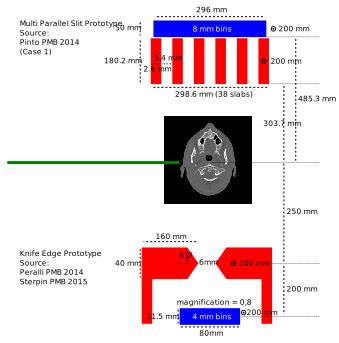
\includegraphics[width=0.9\linewidth]{detectors}
  \caption{Schematic presentation of the two PG cameras considered in this study. The green arrow represents the proton beam. In red the collimation elements and in blue detection elements. The dimensions were taken from \cite{Pinto2014a} and \cite{Perali2014,Sterpin2015}. Note that the two cameras have an identical detector height ($\odot$ symbol), the two cameras were positioned at an identical location above the head during all simulations, and that here they are not drawn to scale.}
  \label{fig:detectors}
\end{figure}

Regarding background ToF selection, for the IBA C230 accelerator with a period of 10 ns, \cite{Pinto2014a} chose a window of 4 ns around the PG maximum, based on experimental ToF spectra. This means that about 60\% of the noise could be removed. For the KES prototype ToF is not used, leading to a higher background, as is evident when one compares the backgrounds as published in the two publications. A second difference is the energy selection window. The IBA group employ a 3-6 MeV window, whereas the CLaRyS collaboration produced their optimization with a 1-8 MeV window. We will compare each camera with their published properties, that is to say: a 1-8 MeV window and ToF for MPS and a 3-6 MeV window without ToF for KES.

Both PG camera prototypes have different photodetectors and different detector electronics. In this study, these differences are not implemented. Instead, the method as described in \cite{Gueth2013} was used to obtain the interaction point of an impinging photon. If the integrated energy deposited in a crystal lies in the acceptable energy and ToF window, the event is recorded. The position of the event in the crystal is considered as the energy weighed barycenter of all interactions in the crystal, plus a random value taken from a 5mm FWHM Gaussian to simulate the electronics and the detector resolution.

\subsubsection{Background modeling}

Background estimation in PG simulation is a difficult and largely unsolved issue \citep{Huisman2016,Sterpin2015,Pinto2014a,Perali2014}. Simulations would ideally include beam nozzle and whole room modeling, but these are habitually omitted. ToF selection techniques can improve the signal-to-noise ratio (SNR) \citep{Testa2008,Roellinghoff2014a}, but then depend on the proper simulation of the beam accelerator time structure. As noted in \cite{Huisman2016}, no validation for background in PG simulations has been performed at this time. In this study, the stable time structure of current generation cyclotrons was assumed, in which the neutron background is largely constant. 

Estimates of background counts in the detector are taken from \cite{Pinto2014a,Perali2014}, which are both based on measured data:

\begin{itemize}[noitemsep]
\item MPS: \cite{Pinto2014a} fig.~9: $1 \cdot 10^{3} \pm 1 \cdot 10^{2}$ per $4\cdot10^9$ primary protons per 8 mm bin
\item[] Converted to per primary proton: $2.5 \cdot 10^{-7} \pm 0.25 \cdot 10^{-7}$
\item KES: \cite{Perali2014} fig.~11: $5 \cdot 10^{-7} \pm 0.5 \cdot 10^{-7}$ per primary proton per 4 mm bin
\end{itemize}

Per unit of bin length, the background yield of the MPS with ToF is therefore 4 times as low as the background seen with the KES. In the context of the fair comparison, for the KES camera the background with ToF can be obtained by multiplying the background with the same $\frac{4 ns}{10 ns} = 0.4$ fraction as with the MPS.

\subsubsection{Beam and target}

We use the test-case presented in \cite{Perali2014} as the KES detector properties such as background were published for that scenario, again in order to remove any doubt that a difference in camera performance could be due to a difference in implementation or setup. A 160 MeV mono-energetic proton beam is shot into a cylindrical PMMA phantom (length 30 cm, radius 15 cm). Employing the batch method we realize 50 simulations for each experiment.

%%%%%%%%%%%%%%%%%%%%%%%%%%%%%%%%%%%%%%%%%%%%%%%%%%%%%%%%%%%%%%%%%%%%%%%%%%%%%%%%
\subsubsection{AMV-specific alterations to setup}

% Since we are using a simulation for the validation of the theoretical expressions in table~\ref{GeomFormulas}, for the fairest comparison possible, we can equalize certain aspects which might cause one camera or the other to give favorable impression. In principle this comparison is not about absorption materials, acquisition electronics or PG selections, but PG collimator characteristics. So, for the validation of the expressions in table~\ref{GeomFormulas} and comparison on LCE, SR and FRP we set the absorber material of the MPS to that of the KES: LYSO. The energy and ToF selection windows are kept identical for both cameras, and are varied in order to study their impact on the figures of merit.

In the case of simulation for analytical model verifications, we use identical absorbers for both prototypes, namely the absorber of the KES prototype and we apply the same energy and TOF selection: the same energy selection ($E> 1~MeV$) and the same TOF selection (no TOF selection).

Note that these two studies will provide information on the influence of TOF and energy selection on the cameras. Indeed, only one parameter will change from the setup used for AMV to the setup for prototypes comparison:
\begin{itemize}
	\item TOF for MPS
	\item Energy selection for MPS
\end{itemize}

Table~\ref{table:FOM} gives an overview of the main cameras parameters used for AMV and prototypes comparison.

\begin{table}
\centering
\begin{tabular}{|l|l|l|l|}
	\hline
	\multicolumn{2}{|c|}{}& 	Analytical model verification & Prototypes comparison\\
	\hline
	Absorber				& MPS & \multicolumn{2}{c|}{LYSO} \\
									& KES & 	\multicolumn{2}{c|}{} \\
	\hline
	Energy & MPS & \multirow{2}{*}{>1 MeV}			&		>1 MeV						\\
	\cline{2-2}\cline{4-4}
	selection				& KES & & 3--6 MeV \\
	\hline	
	TOF & MPS & \multirow{2}{*}{no TOF}			&		TOF						\\
	\cline{2-2}\cline{4-4}
	selection				& KES & & no TOF \\
	\hline		
\end{tabular}
\caption{Summary of the main cameras parameters used for AMV and prototypes comparison.}
\label{table:FOM}
\end{table}

For the AMV, we use the same background level for MPS as the one of KES for the following reason: the background level in the MPS camera is derived in \cite{Pinto2014a} from measurements with large detectors by assuming that the background is proportional to the detector volume. If we apply the same approach, it is reasonable to use the same background levels since we use the same absorbers for MPS and KES. One can argue that the MPS and KES collimators are different. It is true and it is difficult to say whether the larger amount of material in the CLaRyS MPS collimator leads to a larger background with more neutron-induced gammas or a lower background due to a larger attenuation of these gammas\dots At first order the background levels should be similar and a first order estimate is sufficient for a paper that mainly aims at comparing the signal detection of the two cameras.
\todo{Question to Etienne: we discussed that for detection yield, we would not use the background. Then we should here explain clearly for which fig. of merit we use which background, and why. Agreed?}

%%%%%%%%%%%%%%%%%%%%%%%%%%%%%%%%%%%%%%%%%%%%%%%%%%%%%%%%%%%%%%%%%%%%%%%%%%%%%%%%
\subsection{Figures of merit}\label{figmerit}

% The previous paragraph refers to the verification of our simulations and data analysis by comparing the FOP with the results published in Perali, right ? It is presented in Appendix
%, each resulting in a FOP estimate, giving us a mean $\upmu_\textrm{FOP}$ and a standard deviation $\upsigma_\textrm{FOP}$ for a certain experiment. Since we are studying the effect of replacing the CT with a RPCT to simulate patient change, we run each experiment with both CT and RPCT. Each FOP estimate of the N CT realizations is compared to each FOP estimate of the N RPCT realizations, resulting in N$\times$N possible \emph{FOP shift} measurements. These distributions have a $\upmu_\Delta$ and a $\upsigma_\Delta$. The shift initially obtained with the dose is denoted $\Delta_\textrm{dose}$


% Grading the performance of the detectors will be done according to these figures of merit: 

%\begin{itemize}[noitemsep]
%\item Accuracy: $| \upmu_{\Delta} - \Delta_\textrm{dose}|$.
%\item Precision: $\upsigma_\Delta$. For this estimate of the standard deviation of the Gaussian distribution a standard deviation can be computed once again based on the number of realization $n$ used to obtain it: $\upsigma(\upsigma_\Delta)=\frac{\upsigma_\Delta}{\sqrt{2\times(n-1)}}$, as per \citet[formula 4.54]{Leo1994}.
%\item Confidence: the percentage of RPCT FOP realizations that fall outside $\upmu_\textrm{FOP,CT}\pm2\upsigma_\textrm{FOP,CT}$ indicates the likelihood any difference from the expected FOP is measured. In other words, given that in this analysis we know that a shift should be detected, what is the probability that a particular realization does so? It will be denoted as P$_\Delta$.
%\end{itemize}

% \begin{table}
% \centering
% \begin{tabular}{lllll}
% 	\midrule
% 																& Analytical	& Monte Carlo \\
% 	\midrule
% 	\mr{2}{Efficiency}		& MPS		& \mr{2}{LCE}	& 
% 												& KES 				
% 	\midrule
% \end{tabular}
% \caption{Figures of merit.}
% \label{tab:FOM}
% \end{table}



\subsubsection{Analytical Model Verification}

\paragraph{Detection efficiency (DE)}

We can compare the detection efficiency of camera unit with two MC estimates:
\begin{itemize}
	\item the detection yield of a camera unit defined as the ratio of the mean number of detected gammas over the number of emitted gammas for camera units seeing the PG profile,
	\item the contrast of the PG falloff.
\end{itemize}
The two quantities are strongly correlated. The former directly corresponds to the definition of the anaytical detection efficiency $DE_{cu}$ the latter accouts for the partial collimator transparency and it is the camera endpoint in the context of ion-range verification.
\todo{we must mention which background we use here.}

\paragraph{Spatial resolution (SR)}
 The BP is as sharp as it can be in such a scenario, and any blur seen in the detected PG profile is then due to the collimator design. The MC estimate of the PG profile will be performed by computing the first derivative of the PG profile that measuring the FWHM of the resulting peak.

\paragraph{Analytical model and MC comparison}

The analytical model is perhaps best used to understand the relative performances of the collimator designs. The goal is not to produce a good analytical model, but rather to have a tool that makes and informed prediction, supported by MC data. To understand the collimator performances, we will mainly compare ratios the DE and SR values with the two cameras.

Table~\ref{table:FOM} presents the figures of merit used for the analytical model verification.

\begin{table}
\centering
\begin{tabular}{|l|l|c|c|}
	\hline
						& Analytical & \multicolumn{2}{c|}{ MC}\\
	\hline
	Detection efficiency	& $DE_{cu}$	& Detection yield & Contrast \\
	\hline
	Spatial resolution & $s_e$								& \multicolumn{2}{c|}{Fall-off width}\\
	\hline	
\end{tabular}
\caption{Figures of merit for the analytical model verification. Detection yield (under MC) refers to the \emph{signal} detection yield.}
\label{table:FOM}
\end{table}


\subsubsection{Prototype Comparison}

In the comparison of the nominal (unequalized) prototypes, we also take a look at the figures of merit (summarized in table~\ref{table:FOM}). In addition, because of its clinical relevance, the fall-off retrieval precision ($FRP$) will be determined. The FRP is the standard deviation of the FOP, which is obtained by way of the batch method. Each of these can then be examined as function of the energy and ToF selections.

\section{Results}

\subsection{Analytical Model Verification}

\begin{table}
\centering
\begin{tabular}{lllll}
	\midrule
	                            & MPS                              & KES \\
	\midrule
	Effective slit width ($s_e$)& $s$                              & $s + \frac{ln(2)}{\mu~tan(\alpha)}$ \\
 	Det. unit FOV               & $s(1+\frac{d_1}{D})$             & $s_e(1+\frac{d_1}{d_2})$ \\
 	Lin. collection efficiency  & $\frac{H s}{ 4 \pi L D } (1-f) $ & $\frac{H s}{ 4 \pi L d_2 } (1 + x^2/d^2_2)^{-3/2} $ \\
 	Effective thickness ($T_e$) & $D_f$                            & $T$ \\
	\midrule
\end{tabular}
\caption{MPS and KES detection efficiencies and spatial resolution from analytical models. The parameters of the cameras are defined in figure~\ref{GeomSchemes}.}
\label{GeomFormulas}
\end{table}

\begin{table}
\centering
\begin{tabular}{lllll}
	\midrule
	                            & MPS MC & MPS AM & KES MC & KES AM \\
	\midrule
 	Spatial resolution               & $s(1+\frac{d_1}{D})$             & 14.52 mm
 	 & $s_e(1+\frac{d_1}{d_2})$                                    & 13.5 mm\\
 	Efficiency  & $\frac{H s}{ 4 \pi L D } (1-f) $ & $4.18 \cdot 10^5$
 	 & $\frac{H s}{ 4 \pi L d_2 } (1 + x^2/d^2_2)^{-3/2} $         & $6.67 \cdot 10^5$ \\
 	\midrule
\end{tabular}
\caption{MPS and KES detection efficiencies and spatial resolution from analytical models. The predictions of the analytical model (AM column) are given in table~\ref{GeomFormulas}.
TODO: put in correct MC data, but first wait for decision on which selection to take.}
\label{AMVResults}
\end{table}

\begin{table}
\centering
\begin{tabular}{lllllllll}
	\midrule
	Time selection 					& ToF &     &     &     & none&     &     &     \\
	Energy selection 				& 1   &     & 3   &     & 1   &     & 3   &     \\
	Camera 							& MPS & KES & MPS & KES & MPS & KES & MPS & KES \\
	\midrule
 	FOW                         	& 19.7& 20.9& 18.3& 19.3& 19.8& 21.9& 17.9& 23.6\\
 	FOW (perfect collimator) 	& 17.8& 13.7& 16.9& 13.7& 18.3& 14.2& 17.0& 11.6\\
	\midrule
\end{tabular}
\caption{FOW PSF.}
\label{FOWCOMP}
\end{table}

The FOW shown in table~\ref{FOWCOMP} shows that both cameras perform similar with ToF selection. For the MPS the ToF selection makes no difference (up to 2\%), while for the KES it gives a 10-20\% improvement. The results are a bit worse than the calculated values in table~\ref{GeomFormulas}, but close to the 20 mm as postulated in \cite{Priegnitz2015}.

When we make the collimator perfectly absorbing (we kill any tracks entering the material), we can see the KES's effective slit width in action: the transmission through the collimator creating a wider $s_e$ is gone and we see the FOW decrease between 40 and 100\%. This is roughly in line with the calculated $s_e$: \textcolor{red}{ETIENNE?} Surprisingly the FOW of the KES approaches the theoretical value nearly, while the MPS is still a few millimeters worse than calculated.

\begin{itemize}
  \item Formulas of the the MPS and KES detection efficiencies and spatial resolution from analytical models (figure~\ref{GeomFormulas})

  \begin{itemize}
    \item Draw some conclusions about the intrinsic features of MPS and KES collimators knowing that the falloff retrieval precision (FRP)   
    \begin{itemize}
      \item Efficiency: same efficiency with the same $s, L, H$, $d_2(\text{KES}) = D(\text{MPS})$, $d_2(\text{MPS})=0$ (no space between collimator and absorber in MPS) and $f\longrightarrow0$ (perfect collimator). In practice, $f\ne 0$ ($f=0.4$ in the CLaRyS MPS camera) so that the KES camera has a slightly larger efficiency than the MPS camera with the aforementioned geometrical conditions. It is worth noting that the KES detection efficiency is not constant over the FOV.
      \item Spatial resolution: same resolution with the same geometrical conditions and perfect collimators. In practice, MPS transparency can be neglected in the CLaRyS prototype ($D = 180$~mm) but not the KES transparency so that the KES camera has a slightly poorer spatial resolution than the one of the MPS camera (still with the aforementioned geometrical conditions).
    \end{itemize}       
    \item Estimate the MPS and KES performances in Smeets 2016 and Lin 2017: the KES/MPS detection efficiency ratio is 1.6 for Smeets 2016 and 5.3 for Lin 2017 (assuming the use of the same energy window) $\Rightarrow$ these comparisons were unfair\dots   
  \end{itemize}
\end{itemize}

\begin{figure}[htp]
  \centering
  \subfloat[Smeets 2016 setup]{\label{SmeetsComparison}
\includegraphics[width=.45\textwidth]{Smeets2016}}\quad
  \subfloat[Lin's setup]{\label{LinComparison}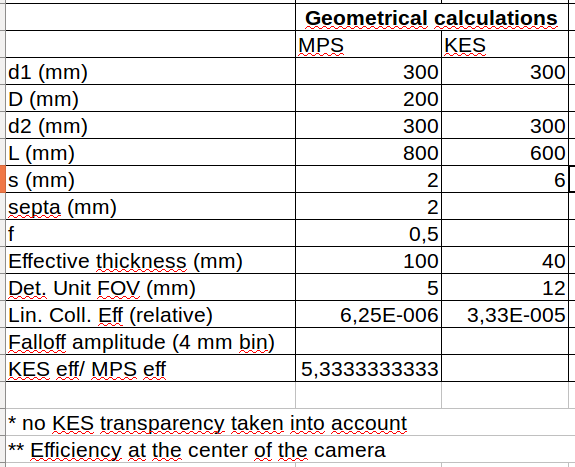
\includegraphics[width=.45\textwidth]{LinComparison}}
  \caption{\label{LitteratureComp} MPS and KES comparisons in litterature.}
\end{figure}   

( \cite{Roellinghoff2014a} shows impact of TOF )



\textcolor{red}{I think it would be better to show PG profiles with 1-8 MeV energy selection with no TOF selection. The advantage of these selections is that it allows us to show the impact of energy (>1 MeV vs 3-6 MeV selection for KES) and TOF selection (for MPS) when we move to the prototypes configurations. We can put in the table of Figure~\ref{CameraPerformancesFairComp} the result with the 3-6 MeV energy selection to show that the results do not depend on energy selection).}

Figures~\ref{PGprofileFairComp} and \ref{CameraPerformancesFairComp}.

\begin{figure}[!htp]
  \centering
  \subfloat[MPS]{\label{SmeetsComparison}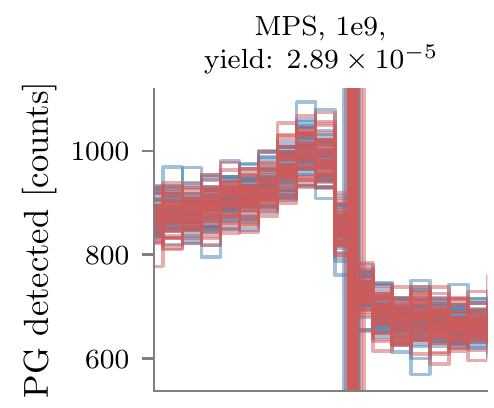
\includegraphics[width=.45\textwidth]{MPS_3-6MeV_noTOF}}\quad
  \subfloat[KES]{\label{LinComparison}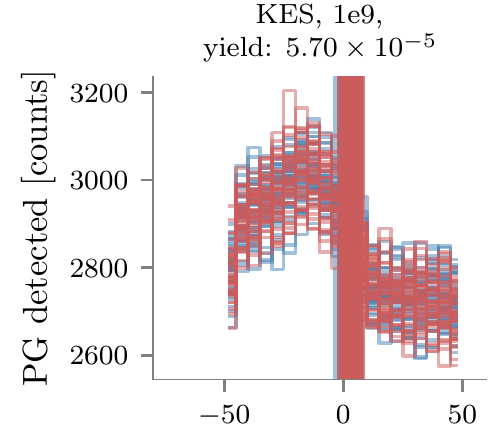
\includegraphics[width=.45\textwidth]{KES_3-6MeV_noTOF}}
  \caption{\label{PGprofileFairComp} MPS and KES comparisons with the same absorber and the same energy (3-6~MeV) and TOF selection (no TOF selection). \textcolor{red}{Sum the statistics of the various 1e9 PG profiles to get the smoothest profiles (we are interested in PG profile shapes). This will allow us to better estimate the falloff features, namely amplitude and width. Put the 2 PG profiles on a single figure?}}
\end{figure}  

\begin{figure}[htp]
  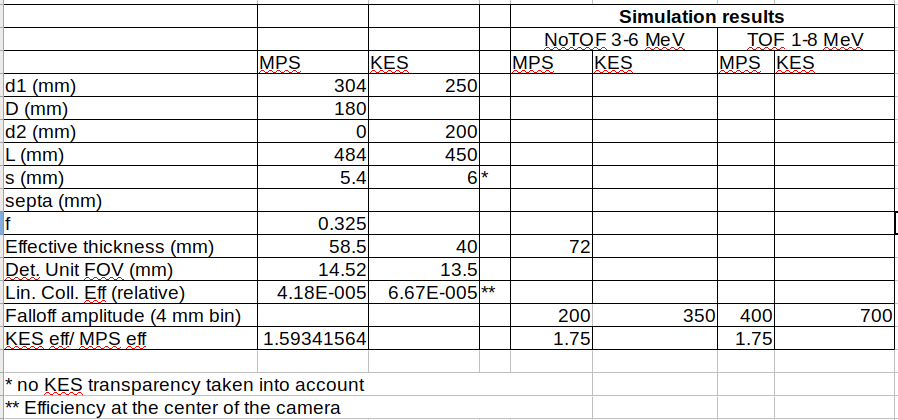
\includegraphics[width=\textwidth]{FairComparison}
  \caption{\label{CameraPerformancesFairComp} MPS and KES comparisons with the same absorber, energy and TOF selection. The first columns of the table correspond to the geometrical calculations. \textcolor{red}{It is interesting to show the results for the two energy selections but it would be nice to have only one TOF selection (no TOF).}}
\end{figure}

\subsection{Prototype Comparison}

Performance under clinical conditions is the eventual purpose of these PG cameras, and therefore we here include the results of the clinical case study. Since both cameras prototypes were optimized assuming their particular choice for absorber and energy selection window, here we chose to set 

\subsubsection{PG profiles}

Figure~\ref{PGprofileProtoComp}.

\begin{figure}[!htp]
  \centering
  \subfloat[MPS]{\label{SmeetsComparison}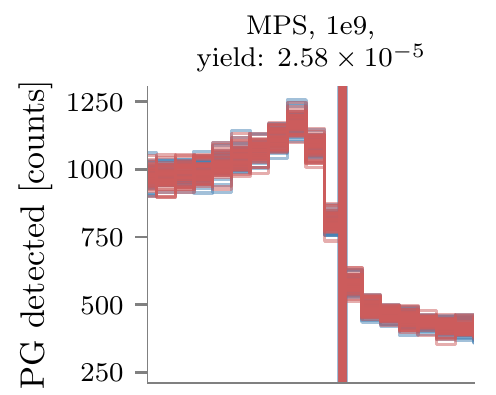
\includegraphics[width=.45\textwidth]{MPS_1-8MeV_TOF}}\quad
  \subfloat[KES]{\label{LinComparison}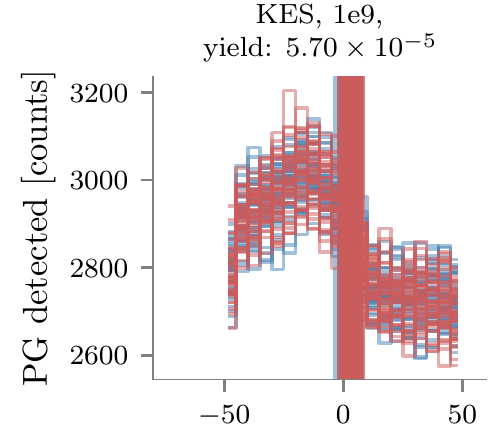
\includegraphics[width=.45\textwidth]{KES_3-6MeV_noTOF}}
  \caption{\label{PGprofileProtoComp} MPS and KES prototypes comparisons. MPS BGO aborber with 1-8 MeV energy selection and TOF selection. KES: LYSO absorber with 3-6 MeV and no TOF selection). \textcolor{red}{Sum the statistics of the various 1e9 PG profiles to get the smoothest profiles (we are interested in PG profile shapes). This will allow us to better estimate the falloff features, namely amplitude and width. Put the 2 PG profiles on a single figure?}}
\end{figure}  

KES/MPS ratio $\sim 400/350 \sim 0.9$.

\subsubsection{FRP}

Figure showing the falloff retrieval precision (FRP) (standard deviation of the falloff position distributions) for the 2 prototypes as a function of the number of incident protons ($10^7$, $10^8$, $10^9$).

\textcolor{red}{We do not have this figure yet. The figure in the spot grouping paper shows the mean and standard deviations on the falloff position differences for the 3 spots considered. }

%%%%%%%%%%%%%%%%%%%%%%%%%%%%%%%%%%%%%%%%%%%%%%%%%%%%%%%%%%%%%%%%%%%%%%%%%%%%%%%%
\section{Discussion}


%%%%%%%%%%%%%%%%%%%%%%%%%%%%%%%%%%%%%%%%%%%%%%%%%%%%%%%%%%%%%%%%%%%%%%%%%%%%%%%%
\section{Conclusion}


%%%%%%%%%%%%%%%%%%%%%%%%%%%%%%%%%%%%%%%%%%%%%%%%%%%%%%%%%%%%%%%%%%%%%%%%%%%%%%%%
\section{Acknowledgements}

This work was partly supported by SIRIC LYric Grant INCa-DGOS-4664, LABEX PRIMES (ANR-11-LABX-0063 / ANR-11-IDEX-0007) and Fondation ARC. The authors would like to thank Marie-Claude Biston, Thomas Baudier and Gloria Vilches-Freixas for their help finding the CT images and making the treatment plan. We also thank Erik Almhagen and Uppsala University Hospital, Sweden for the treatment plan data presented in this paper.

%%%%%%%%%%%%%%%%%%%%%%%%%%%%%%%%%%%%%%%%%%%%%%%%%%%%%%%%%%%%%%%%%%%%%%%%%%%%%%%%
\newpage

\appendix
% \begin{appendices}
% 
%%%%%%%%%%%%%%%%%%%%%%%%%%%%%%%%%%%%%%%%%%%%%%%%%%%%%%%%%%%%%%%%%%%%%%%%%%%%%%%%

\section{Fall-off position and width estimation procedure}\label{sec:fopproc}

\subsection{Fall-off position estimation procedure}

From a clinical perspective, the range estimate could be more interesting than FOP, because it can distinguish simple offset errors from patient morphological change. While the MPS camera was conceived for whole range PG profile detection, the KES camera FoV was chosen for BP region PG detection only. To make the comparison fair, only the FOP could be considered. Multiple approaches to extracting a FOP from the line profile have been proposed \citep{Smeets2012,Gueth2013,Roellinghoff2014a,Janssen2014,Sterpin2015}. In preparatory work, a number of the proposed procedures were investigated. Significant sensitivity to free parameters on the final FOP estimates were seen. In summary, the FOP estimate depends greatly on the procedure, and often on having yields uncommon on the spot-level in clinical TPs, and also on an absence of unavoidable inhomogeneities.

Therefore the fitting method was not chosen as a topic for study in this paper. Instead, a simple method that works on most the data available to the authors was used: first a smoothed and interpolated spline function is fitted against the detected PG data points, after which a baseline and (distal) peak position are determined. The intersection of the spline with the half-height of the peak above the baseline is then taken as the FOP. A more detailed description of the procedure may be found in appendix~\ref{sec:fopproc}.


\begin{enumerate}[noitemsep]
\item The measured PG profile is smoothed and interpolated with a smoothing spline function:

\begin{equation}
\sum_{i=1}^n (y_i - \hat f(x_i))^2 + \lambda \int_{x_1}^{x_n} \hat f''(x)^2 \,dx
\end{equation}

where $y_i$ is the measured PG profile and $x_i$ the associated x-coordinates, $\hat f(x_i)$ the estimate smoothed spline function and $\lambda$ a smoothing parameter that determines the penalty for deviating from measurement in exchange for smoothness (second order derivatives are close to zero on smooth functions). $\lambda = 0$ produces a perfect spline fit to the data, while $\lambda \gg 1$ produces a horizontal line. We found that $\lambda = 2$ provided an acceptable trade-off between overfitting to noise and removing too many features, which tends to happen for low statistic measurements.
\item The obtained function is plotted for 1024 $x_j$, an number that provided a sufficiently high resolution. Any $f(x_j) < 0$ are set to $0$. 
\item The global maximum is found.
\item The baseline is set equal to the lowest 25\% of bins.
\item From the distal end backwards, the first maximum is taken as the distal most peak position, if it is above the threshold of 30\% of the difference between baseline and global maximum. If no such point is found, the global maximum is taken as the distal most maximum.
\item The fall-off amplitude (FOA) is set to the difference between the distal maximum and baseline: $FOA = max-baseline$. The FOP is obtained by traversing the smoothed profile from the distal end towards the peak until $y_j > \frac{1}{2}FOA$.
\end{enumerate}

The results of this procedure are illustrated in figure~\ref{fig:our-fit}. Every PG profile was estimated 50 times, and so we obtained 50 estimates for the FOP. It is assumed that the FOPs follow a Gaussian distribution, so the mean of the 50 realizations gives the best FOP estimate and the sigma gives the precision of the ability to estimate the best FOP. Comparing the 50 FOP estimates obtained from the CT with the 50 estimates obtained from the RPCT simulations, gives 2500 possible shift estimates. Again, the distribution of shifts should be centered at the true shift, while the sigma indicates how likely it is that this true shift is detected under the current conditions.

\begin{figure}[htp]
  \centering
  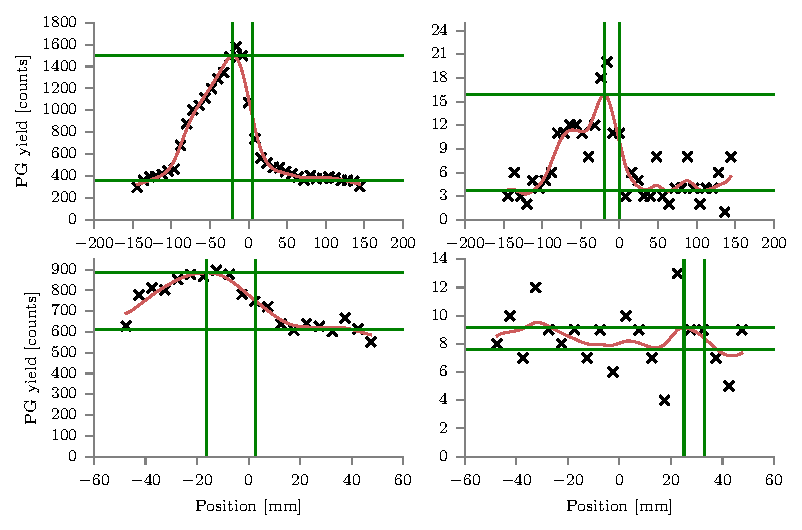
\includegraphics[width=0.9\linewidth]{fopproc}
  \caption{The top row demonstrates the fall-off determination procedure on the multi-parallel camera data; on the bottom row on knife-edge slit camera data. The left column is produced with a PG signal due to $10^9$ primaries, while the right column was produced with $10^7$ primary protons. In black crosses the measured PG counts are plotted. The smoothed data is shown in red. The green horizontal lines are drawn at the obtained distal maxima and baselines, while the vertical green lines shown the position of the distal maximum and the position of the fall-off. For the bottom-right plot, a history is visible where the procedure fails: the background induces an erroneous peak detection.}
  \label{fig:our-fit}
\end{figure}

\subsection{Fall-off width estimation procedure}

\begin{figure}[htp]
  \centering
  \subfloat[KES]{\label{FOWKES}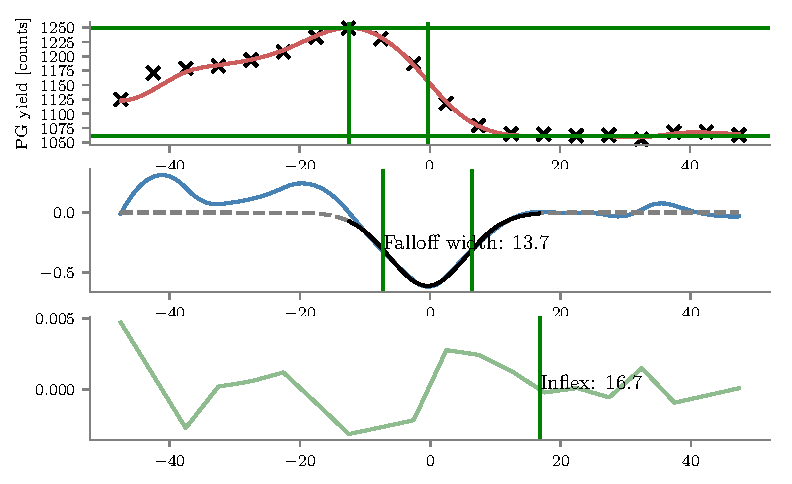
\includegraphics[width=.45\textwidth]{FOW_PMMA_phantom-iba-auger-tof-3}}\quad
  \subfloat[MPS]{\label{FOWMPS}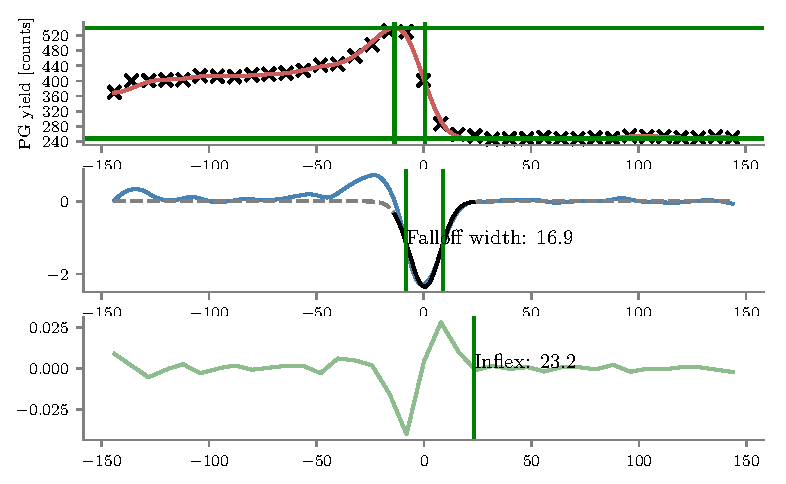
\includegraphics[width=.45\textwidth]{FOW_PMMA_phantom-ipnl-auger-tof-3}}
  \caption{\label{FOWILLUS} MPS and KES FOW estimation illustrated.}
\end{figure}

Figure~\ref{FOWILLUS} shows and illustration of the procedure for two selected profiles obtained with each collimator. To estimate the fall-off with FOW, we smooth the profile in a similar manner as for the FOP estimation, as detailed in appendix~\ref{sec:fopproc} (row 1 in fig.~\ref{FOWILLUS}). Then, a first and second order derivative is computed. On the first order derivative, a Gaussian is fitted (dashed line on second row), on the interval (solid line) between the profile maximum (Bragg Peak) and the first inflection point past the FOP on the second order derivative (here the 1D PG profile is at the baseline of the background, see third row). The Gaussian is fit with a fixed offset of zero, because the baseline of the background is zero. The full width half max of the fitted Gaussian is then taken as the FOW (second row).

%%%%%%%%%%%%%%%%%%%%%%%%%%%%%%%%%%%%%%%%%%%%%%%%%%%%%%%%%%%%%%%%%%%%%%%%%%%%%%%%

\section{Verification of the cameras}

In \cite{Priegnitz2015} PG shifts due to beam energy shifts are studied for the KES camera: the \emph{detectability} of the fall-off as function of the number of primaries. Here that simulation was recreated: a mono-energetic beam shoots into a waterbox at two energies. 50 realizations are generated with a 139 MeV beam energy, and 50 realizations with 144 MeV. At $10^9$ primaries, the distributions are well separated with a shift of 8.3 mm (different from \cite{Priegnitz2015} because of the different material). In figure 13 in \cite{Perali2014} with $10^9$ primaries a standard deviation of 1.5 mm is obtained, while here 1.21 and 1.14 mm were obtained. It is sufficient agreement to be confident of our setup and further results.

The KES prototype's sensitivity to accurate positioning with respect to the expected FOP was elaborated upon in \citet[Section IV.A.3]{Sterpin2015}: the detector response is, due to the KES collimator, not linear as with a parallel slit collimator. In this study, to make the comparison as fair as possible and avoid any bias, alignment on the FOP specific for each spot was ensured as follows: the intermediate PG source image of vpgTLE (equivalent to the PG emission) was projected on the beam axis, and then convolved with a Gaussian of $\upsigma = 8.5$ mm, which corresponds to the point spread function (PSF) with a FWHM of 20 mm used in \cite{Priegnitz2015} to approximate the detected profiles from the emitted profile. These profiles will be referred to as "PG + PSF" profiles. As a matter of fact, the MPS prototype has roughly the same PSF as the KES prototype so that "PG + PSF" fall-off position can be considered as the expected position for both cameras.

To verify the implementation of the MPS camera, the precision on the FOP, obtained with the procedure outlined in the previous paragraph, is compared to earlier results. In the caption of figure 9 in \cite{Pinto2014a} it is stated that with $10^8$ primaries a standard deviation of 1.3 mm is obtained for the detector design used here, which is about 20\% different from the results obtained in this study: 1.63 and 1.54 mm.
%%%%%%%%%%%%%%%%%%%%%%%%%%%%%%%%%%%%%%%%%%%%%%%%%%%%%%%%%%%%%%%%%%%%%%%%%%%%%%%%
% \end{appendices}
\newpage

%%%%%%%%%%%%%%%%%%%%%%%%%%%%%%%%%%%%%%%%%%%%%%%%%%%%%%%%%%%%%%%%%%%%%%%%%%%%%%%%

\bibliographystyle{plainnat}
\bibliography{lib.bib}
\end{document}%\grid
